\chapter{Introducción}

El desarrollo de tecnología es un aspecto estratégico para un país en vías de desarrollo, así lo han demostrado otras naciones que han visto que la tecnología no solo tiene consecuencias económicas, sino que que también contribuye a elevar la calidad del conocimiento en la sociedad, afectando de forma significativa la vida de sus habitantes.

La robótica corresponde a un área tecnológica que ha escalado rápidamente, desde los primeros robots manipuladores instalados en cadenas de producción por los años de 1960, hasta hoy en día donde ya es una realidad poder interactuar usando lenguaje natural con un robot domestico.

Los robots ya no solo han están supeditados a una sección de una fabrica donde operan la misma rutina una y otra vez, nuevos avances han hecho que los robots sean  capaces de percibir el ambiente y poder trabajar junto a las personas. Muchas veces se han convertido en una extensión de nosotros mismos, ejemplo de ello es el robot Da Vinci, que permite ejecutar movimientos de alta precisión y control permitiendo cirugías de invasividad mínima.

Sin duda los robots han desplazado al humano en muchas tareas, algunas de estas se desarrollan en ambientes hostiles y peligrosos, así han convertido al trabajador en operador, aumentando de forma significativa su seguridad. Este tipo de robots se denominan teleoperados, pues pueden ser operados a distancia por el usuario.

Es en este marco de robots teleoperados donde se contextualiza el presente trabajo de memoria, pues existen una serie de procesos pueden ser llevados a cabo usando robots teleoperados reduciendo de el riesgo asociado en la operación.

\section{Motivación}

La industria minera en Chile es una de las principales actividades de la economía, representando cerca del 9\% del PIB \cite{sofofa}. Representa una oportunidad de desarrollo tecnológico y es esto lo que permitirá mantener al país como el principal productor de cobre a nivel mundial.

Parte importante explotación minera se realiza de forma subterránea, donde el ambiente de trabajo es peligroso y se deben extremar las medidas de seguridad para resguardar la integridad de los trabajadores. Una de las tareas realizadas en minería consiste en la fragmentación de rocas usando un martillo hidráulico operado de forma local.

La operación de este dispositivo de forma remota y desarrollar algoritmos que permitan su operación autónoma es una tarea compleja, que involucra una serie de etapas, la primera de ellas sería realizar pruebas de concepto en un equipo a escala que permita el desarrollo de sistemas de teleoperación y posterior automatización. Es en este tema donde en enmarca el objetivo principal de este trabajo de memoria.

\section{Objetivos}

A continuación se describen los distintos objetivos y alcances en el desarrollo del proyecto, junto con el esquema de planificación que se desea llevar a cabo.

\subsection{Objetivo General}

Teleoperación háptica en tiempo real de manipulador robótico Scorbot ER VII, basado en la interfaz Phantom Omni y bus de campo EtherCAT, para aplicaciones de automatización de robot picarocas usados en minería.

\subsection{Objetivos específicos}

\begin{itemize}

\item Implementación de servo controladores usando el bus de campo EtherCAT basado en microcontroladores industriales XMC y controladores de motores de Infineon.

\item Integración del sistema en ROS empleando el framework de planificación MoveIt!

\item Implementación de un sistema de teleoperación háptica usando la interfaz Phantom Omni.

\item Evaluación del desempeño del sistema considerando aplicaciones para robot picarocas usados minería.

\item Desarrollar el software y documentación de forma extensible para permitir su modificación futura.

\end{itemize}


\section{Planificación}

Dado que el desarrollo del proyecto considera elementos de hardware y software, es muy importante definir los tiempos de desarrollo de cada uno de estos elementos. La Figura \ref{cap1_tabla_gantt} muestra una tabla de una carta Gantt con las distintas tareas a desarrollar tanto en software como en hardware.

\begin{figure}[ht]
  \centering
  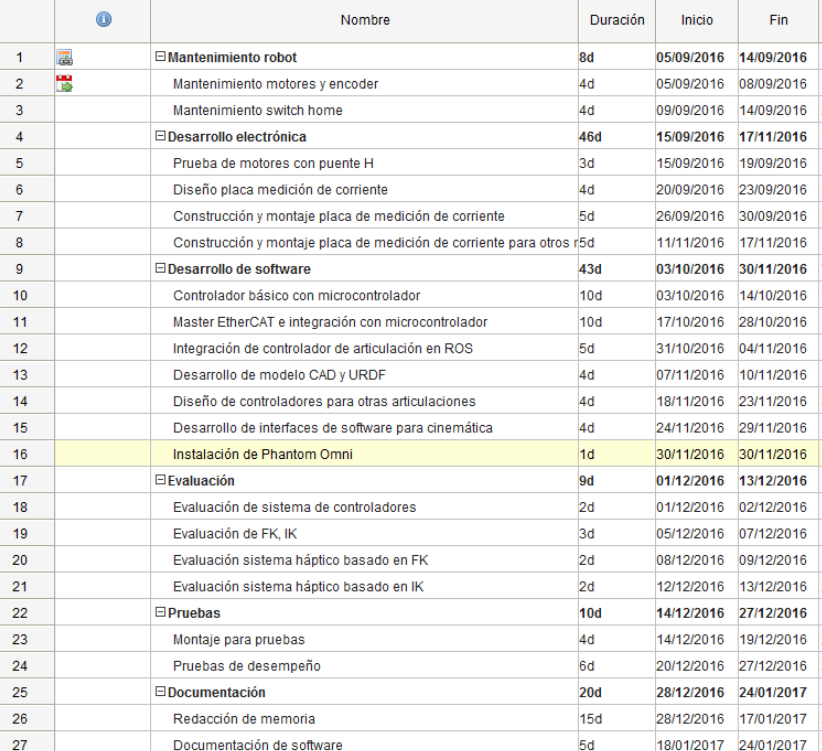
\includegraphics[scale=0.5]{img/cap1/tareas_gantt}
  \caption{Tareas en carta Gantt.}
  \label{cap1_tabla_gantt}
\end{figure}

Uno de los supuestos que presenta la planificación corresponde a que una vez desarrollado un controlador para una articulación, las otras articulaciones tendrán un tiempo de desarrollo mucho más acotado, pues se empleara el ya desarrollado como base.

Se espera que el desarrollo se inicie el 5 de septiembre de 2016 y concluya el 24 de enero de 2017, considerando tiempos de redacción de este documento y documentación asociada.








